\documentclass[12pt]{article}
\usepackage{a4}
\usepackage[english]{babel}
\setlength{\parindent}{0.35cm}
\pagestyle{headings}
\usepackage{graphicx}
\usepackage{grffile}
%Multiple picture in one figure
%\usepackage{subfigure}
\usepackage{subfig}
\usepackage[utf8]{inputenc}
\usepackage{listings}
\usepackage{color}
\usepackage{wrapfig}
%Floating-Umgebungen
\usepackage{float}
%Math-Environment
\usepackage{amsmath}
\usepackage{amssymb}
\usepackage{bbm}
%Better SI-Units
\usepackage{siunitx}
%Using Appendix
\usepackage[title]{appendix}
%Using URL
\usepackage[hidelinks]{hyperref}
%Using Colored Tables
\usepackage{colortbl}
\newcommand{\gray}{\rowcolor[gray]{.90}}
\usepackage{esvect}
% Use fancy tables
\usepackage{tabularx}
% Build fancy tables
\usepackage{booktabs}
% Write pseudo-code
\usepackage{algorithm}
\usepackage[noend]{algpseudocode}
% Configure enumeration
\usepackage{enumitem}
%Configure geometry
\usepackage{geometry}
\geometry{
	a4paper,
	left=3cm,
	right=3cm,
	top=3cm,
	bottom = 3cm,
	}

\lstset{
	language=C++,
	basicstyle=\small\ttfamily,
	keywordstyle=\color{blue}\ttfamily,
	stringstyle=\color{red}\ttfamily,
	commentstyle=\color{green}\ttfamily,
	morecomment=[l][\color{magenta}]{\#},
}


\usepackage{amsthm}

\renewcommand\qedsymbol{$\blacksquare$}
\newtheorem{theorem}{Theorem}[section]

\begin{document}
	
	\title{
		\textbf{\huge{CSE 446: Machine Learning Winter 2018 }} \\[2cm]
		\LARGE{Assignment 4}\\[1cm]
	}
	\author{from \\ Lukas Nies \\ University of Washington}
	\date{\today}
	\clearpage\maketitle\thispagestyle{empty}
	\newpage

	\tableofcontents
	\setcounter{page}{0}
	\newpage
	
	% To start with section 1 labeled as section 0
	\setcounter{section}{-1}
	

\section{Policies}

\subsection{List of Collaborators}

My collaborator was Edith Heiter (discussed parts of Problem 1 an 2). The development of the answers and code though was completely independent and individually.

\subsection{List of Acknowledgments}

None.

\subsection{Policies}

I have read and understood these policies.


\newpage

\section{Convexity: Linear and Logistic Regression}



\begin{enumerate}
	\item If the trainings data is linear separable and we have binary label then the squared error can not converge to 0 since a straight line is not able to fit linear separated binary label. The log loss though is able to approximate the Heaviside function (when weights get large) and therefore is able to converge to zero.
	\item The solution space for under constraint problems ($d\geq n$) is large. If we do not have regularization and the data points are linearly separable then there will be a solution in this solution space that minimizes both the regression problems. Hence, both the squared error and the log loss converge to zero. 
	\item If we hit zero misclassification error we still will be updating our parameters afterwards since we do not optimize the misclassification error but rather the objective function. Even if the error gets zero the parameters can still be optimized to get a better margin. 
\end{enumerate}

\section{Neural Networks and Non-convex optimization}

\subsection{Computational Complexity}

\begin{enumerate}
	\item 
	\begin{algorithm}
		\caption{Forwardpass without mini batches}\label{alg:FWP}
		\begin{algorithmic}[1]
			\Procedure{Forwardpass}{$x$}
			\State $a^{(0)} \gets x$ \Comment{Assign input $x \in \mathbb{R}^{d^{(0)}=d}$ to input nodes}
			\State $z^{(0)} \gets h(a^{(0)})$ \Comment{Compute output $z^{(0)}\in\mathbb{R}^{d^{(0)}=d}$  of input layer}
			\State $w^{(l)} \gets$ initialize\_weigths() \Comment{Initialize all weights $w\in\mathbb{R}^{d^{(l)}\times d^{(l-1)}}$}
			\For{layer $l$ in all layers $L$}\Comment{Iterate over all layers L}
			\State $a^{(l+1)} \gets w^{(l+1)}\cdot z^{(l)}$ \Comment{Calculate activation $a^{(l+1)}\in\mathbb{R}^{d^{(l+1)}}$}
			\State $z^{(l+1)} \gets h(a^{(l+1)})$ \Comment{Calculate output $z^{(l+1)}\in\mathbb{R}^{d^{(l+1)}}$}
			\EndFor
			\State \textbf{return} $\hat{Y} = a^{(L+1)}$ \Comment{Return the target values $\hat{Y}\in\mathbb{R}^{d^{(L+1)}=k}$}
			\EndProcedure
		\end{algorithmic}
	\end{algorithm}	
	\item 
	\begin{algorithm}
		\caption{Forwardpass with mini batches}\label{alg:FWPmini}
		\begin{algorithmic}[1]
			\Procedure{Forwardpass}{$X$}
			\State $a^{(0)} \gets X$ \Comment{Assign input $x \in \mathbb{R}^{m \times d^{(0)}=m\times d}$ to input nodes}
			\State $z^{(0)} \gets h(a^{(0)})$ \Comment{Compute output $z^{(0)}\in \mathbb{R}^{m \times d^{(0)}=m\times d}$  of input layer}
			\State $w^{(l)} \gets$ initialize\_weigths() \Comment{Initialize all weights $w\in\mathbb{R}^{d^{(l)}\times d^{(l-1)}}$}
			\For{layer $l$ in all layers $L$}\Comment{Iterate over all layers L}
			\State $a^{(l+1)} \gets z^{(l)}\cdot \left(w^{(l+1)}\right)^T$ \Comment{Calculate activation $a^{(l+1)}\in\mathbb{R}^{m\times d^{(l+1)}}$}
			\State $z^{(l+1)} \gets h(a^{(l+1)})$ \Comment{Calculate output $z^{(l+1)}\in\mathbb{R}^{m\times d^{(l+1)}}$}
			\EndFor
			\State \textbf{return} $\hat{Y} = a^{(L+1)}$ \Comment{Return the target values $\hat{Y}\in\mathbb{R}^{m\times d^{(L+1)}=m\times k}$}
			\EndProcedure
		\end{algorithmic}
	\end{algorithm}		
	
	\item To compute the squared loss 
	\begin{align}
		\frac{1}{2}\frac{1}{N}\left( Y - \hat{Y} \right)^2
	\end{align}
	one has to calculate the computation time of the forward pass in respect to the mini batch $X$ with size $m$, the input dimension $d = d^{(0)}$, the number of hidden nodes $d^{(1)}\dots d^{(L)}$, the output dimension $k = d^{(L+1)}$, and the cost $C_h$ for computing the transfer function $h(.)$. \par
	Per iteration one has to calculate the dot product of the activation of the previous layer $a^{(l)}$ and the weights $w^{(l+1)}$, therefore we get a computation time of $ \mathbb{R}^{m\times d^{(l)}} \cdot \mathbb{R}^{d^{(l)}\times d^{(l+1)}} \leftrightarrow O\left( md^{(l)}d^{(l+1)}\right)$. We also have to calculate the output of the resulting activation: $O(h(a^{l+1}))\rightarrow O(C_hmd^{(l+1)})$. Combining this gives us a computation time of $O\left( md^{(l+1)}\cdot(C_h + d^{(l)}) \right)$. Now we cum over all layers and get the total computational time:
	\begin{align}
		T = O
			\left(
				\sum_{l=0}^{L} md^{(l+1)}\cdot(C_h + d^{(l)})
			\right)
	\end{align}
	\item According to the Baur-Strassen theorem calculating the backpropagation only takes in the order of five times longer than calculating the forward propagation. Therefore, and because calculating the derivative of the transfer function is in the sam ballpark as calculating the transfer function itself, we get
	\begin{align}
		T \approx 5\times O
		\left(
		\sum_{l=0}^{L} md^{(l+1)}\cdot(C_h + d^{(l)})
		\right)
	\end{align}
	\item We only want to calculate the top level derivative of the neural network then we can just apply the definitions:
	\begin{align}
		\frac{\partial l(y,\hat{y}(X))}{\partial w^{(L+1)}}= \frac{\partial l(y,\hat{y}(X))}{\partial a^{(L)}}\frac{\partial a^{(L+1)}}{\partial w^{(L)}} = - ( y - \hat{y}(X) )^T\cdot z^{(L)}
	\end{align}
	Since we already applied forwardporpagation and stored all the activations and outputs we only have to calculate the dot product $(\hat{y}(X) )^T\cdot z^{(L)}$, this give a computational time of 
	\begin{align}
		T_{\text{partial}} = O\left( md^{(L+1)}d^{(L)} \right) = O\left( mkd^{(L)} \right). 
	\end{align}
\end{enumerate}


\subsection{Saddle Points and Symmetry}

\begin{enumerate}
	\item If we consider a MLP with zero hidden layers (aka perceptron) and if we set all weights to zero then we do not end up in a saddle point. This can be shown by looking at the gradient at the output (dropping indices in the following):
	\begin{align}
		\frac{\partial l(y,\hat{y})}{\partial w^{(1)}}= \frac{\partial l(y,\hat{y})}{\partial a^{(1)}} \frac{\partial a^{(1)}}{\partial w^{(1)}} = - ( y - \hat{y} )\cdot x
	\end{align}
	Since all the weights are initialized with zero, the target function $\hat{y} = w^{(1)}\cdot a^{(0)} = w\cdot x$ vanishes. Therefore the gradient is $-yx$ and hence, we did not initialize in a saddle point.
	\item Consider a MLP with one hidden layer and a $\tanh$ transfer function. Then the gradient at the output layer is given by
	\begin{align}
	\frac{\partial l(y,\hat{y})}{\partial w^{(2)}}&= \frac{\partial l(y,\hat{y})}{\partial a^{(2)}}\frac{\partial a^{(2)}}{\partial w^{(2)}} = - ( y - \hat{y} )\cdot z^{(1)} = - ( y - \hat{y} )\cdot \tanh(a^{(1)}), \\
	\intertext{and the gradient at the hidden layer by}
	\frac{\partial l(y,\hat{y})}{\partial w^{(1)}} &= \frac{\partial l(y,\hat{y})}{\partial a^{(1)}} \frac{\partial a^{(1)}}{\partial w^{(1)}}= - ( y - \hat{y} )\cdot z^{(1)} = - ( y - \hat{y} )\cdot w^{(2)}\cdot \tanh'(a^{(1)}) a^{(0)}
	\end{align}
	The gradient of the hidden layer vanishes since $w^{(2)}$ is initialized as zero, the gradient of the output layer vanishes since $\tanh(a^{(1)})=\tanh(w^{(0)\cdot x})=\tanh(0)=0$.
	We can compute the gradient at the output and an arbitrary layer $l$ for a MLP with more than one layer: 
	\begin{align}
		\frac{\partial l(y,\hat{y})}{\partial w^{(L+1)}}&= \frac{\partial l(y,\hat{y})}{\partial a^{(L+1)}}\frac{\partial a^{(L+1)}}{\partial w^{(L+1)}} = - ( y - \hat{y} )\cdot z^{(L)} = - ( y - \hat{y} )\cdot \tanh(a^{(L)}), \label{eq:MLPtop} \\
		\frac{\partial l(y,\hat{y})}{\partial w^{(l)}} &= \delta^{(l)} z^{(l-1)} = \tanh'(a^{(l)})w^{(l+1)}\delta^{(l+1)}z^{(l-1)} \label{MLParbitrary}
	\end{align}
	All those gradients vanish since all $w$ are zero. Hence, we initialize in a stationary point, hence, a saddle point.
	\item If we now consider the same MLP with a sigmoid transfer function then we look at the generalizations from equations \eqref{eq:MLPtop} and \eqref{MLParbitrary} by exchanging the sigmoid with the $\tanh$. Equation $\ref{MLParbitrary}$ is still vanishing but the gradient in the output layer is non-zero since $sigm(0) = 0.5$ and therefore the gradient is $-\frac{1}{2}y$. Hence, the initialization does not end up in a saddle point. \par 
	If we consider equation \ref{MLParbitrary} we see that, if we update the top layer weights non-zero (since the gradient does not vanish), we get a non-zero weight update in the following layer, and thus, non-zero updates in all the other layers. This is obvious if we plug ins some parameters:
	\begin{align}
		\frac{\partial l(y,\hat{y})}{\partial w^{(L)}} &= \delta^{(L)} z^{(L-1)} = sigm'(a^{(L)})w^{(L+1)}\delta^{(L+1)}z^{(L-1)}\\ &= sigm'(0)(-0.5y)(-(y-a^{(L+1)}))sigm(a^{(L-1)})\\
		&= 0.25y^2 \cdot sigm'(0) = \frac{1}{8}y^2
	\end{align}
	Therefore, if we propagate the weights further back, we can see that the weights depend on the label $y$.
\end{enumerate}

\subsection{Representation and Non-linear Decision Boundaries}

\begin{enumerate}
	\item 
	\begin{enumerate}[label=(\alph*)]
		\item If we use the identity as the transfer function we can rewrite the general rules for the forward propagation
		\begin{align}
			a^{(l+1)} &= w^{(l+1)}\cdot z^{(l)} = w^{(l+1)}\cdot a^{(l)} = w^{(l+1)}\cdot (w^{(l)}\cdot a^{(l-1)}) \\
			&= w^{(l+1)}w^{(l)}\dots w^{(1)}\cdot x \equiv w\cdot x.
		\end{align}
		By redefining the product of all weight vectors to one weight vector we can see the the forward process is just a simple perceptron. The update by the backpropagation algorithm also can be boiled down to a perceptron like form:
		\begin{align}
		\frac{\partial l(y,\hat{y})}{\partial w^{(L+1)}}&= \frac{\partial l(y,\hat{y})}{\partial a^{(L+1)}}\frac{\partial a^{(L+1)}}{\partial w^{(L+1)}} \sim - ( y - \hat{y} )\cdot x \\
		\frac{\partial l(y,\hat{y})}{\partial w^{(l)}} &= \delta^{(l)} a^{(l-1)} = a'^{(l)}w^{(l+1)}\delta^{(l+1)}a^{(l-1)} \sim - ( y - \hat{y} )\cdot x
		\end{align}
		Since this perceptron as convex model has only one global minimum and can represent the same functions as the neural network with the identity as a transfer function we have fulfilled the requirements of the problem. 
		\item 
		We can play the same game but now using a quadratic transfer function
		\begin{align}
		a^{(l+1)} &= w^{(l+1)}\cdot z^{(l)} = w^{(l+1)}\cdot (a^{(l)})^2 = w^{(l+1)}\cdot ((w^{(l)}\cdot a^{(l-1)}))^2 \\
		&= w^{(l+1)}(w^{(l)}\dots w^{(1)})^2\cdot x^2 \\
		&\equiv w\cdot x^2 = w\cdot (x_1^2 + x_2^2 + \cdot + x_d^2 + x_1x_2 + x_1x_3 + \cdot +  x_dx_{d-1}).
		\end{align}
		Wait! This is again a perceptron, but this time with a quadratic feature mapping! Continuing with the backprob we find the same results as above. Therefore we can as well simplify this neural network as a perceptron with quadratic feature mapping. Hence, we have the benefits of a convex model with same capabilities as the neural network.
	\end{enumerate}
	\item
	\begin{enumerate}[label=(\alph*)]
		\item 
		For solving the XOR problem we can use a linear or a quadratic feature mapping. The quadratic mapping is given as follows:
		\begin{align}
			\varphi(x)= 
			\begin{pmatrix}
				x_1 \\ x_1\cdot x_2
			\end{pmatrix}
		\end{align}
		This maps the data points such that the problem can be solved with a single linear decision boundary. In order to solve this problem with a one layer neural network we can use bias terms in combination with the $\tanh$ transfer function the solve this problem.
		\item 
		Writing the forward propagation down for this neural network including bias terms results in the following output
		\begin{align}
			\hat{y}&=\sum_{j=1}^{2}w^{(2)}_j\tanh(a^{(1)}_j) + b \\
			&= w^{(2)}_1 \tanh(w^{(1)}_{11}x_{1} + w^{(1)}_{12}x_{2}+b_1) + w^{(2)}_2 \tanh(w^{(1)}_{21} x_1 + w^{(1)}_{22}x_2 + b_2) +b
		\end{align} 
		Now, if we choose the weights and the bias terms correctly, we can get zero misclassification error of the output function is a $sign$ function.
		I found: 
		\begin{align}
			w^{(1)}_{11} = 2 && w^{(1)}_{12} = 2 && w^{(1)}_{21} = -2 && w^{(1)}_{22} = -2 \notag \\ w^{(2)}_1 = 1 && w^{(2)}_2 = 1 && b_1 = -2 && b_2 = -2 && b = 1
		\end{align}
		If we feed those parameters then we get
		\begin{align}
			\hat{y}(\begin{pmatrix}
				1 \\ 1 
			\end{pmatrix}) &\approx 0.964 \\ 
			\hat{y}(\begin{pmatrix}
			-1 \\ -1 
			\end{pmatrix}) &\approx 0.964 \\ 
			\hat{y}(\begin{pmatrix}
			1 \\ -1 
			\end{pmatrix}) &\approx -0.928 \\ 
			\hat{y}(\begin{pmatrix}
			-1 \\ 1 
			\end{pmatrix}) &\approx -0.928.
		\end{align}
		We can see that, if we apply then $sign$ function, the MLP exactly mimics the XOR function and therefore solves the problem.
	\end{enumerate}
\end{enumerate}

\section{MLPs on MNIST}

\subsection{One hidden layer MLP}

\begin{enumerate}
	\item
	\begin{enumerate}[label=(\alph*)]
		\item 
		For running gradient descent I used pytorch and built a one layer hidden network with 100 hidden nodes, a minibatch size of $200$, trained for $500$ epochs, used a constant step size of $0.1$ and no regularization. The weights are initialized by picking values from a normal distribution between zero and one. 	
		\item 
		For larger stepsizes than $0.1$ or $1$ we do not really find a decrease in error rate. The error does not diverge since we limit our output and the transfers with the sigmoid function which is limited between $0$ and $1$. 	
		\item See figure \ref{fig:sigmoid}
		\item See figure \ref{fig:sigmoid}. The lowest test error achieved is around $5\%$. I think it could have been better if I would have trained it longer but since I ran the code on my Windows laptop on a virtual machine it took some time to even calculate 500 epochs. But for higher epochs we see some overfitting going on so training too long might be a good choice either. 
		\begin{figure}[h]
			\centering
			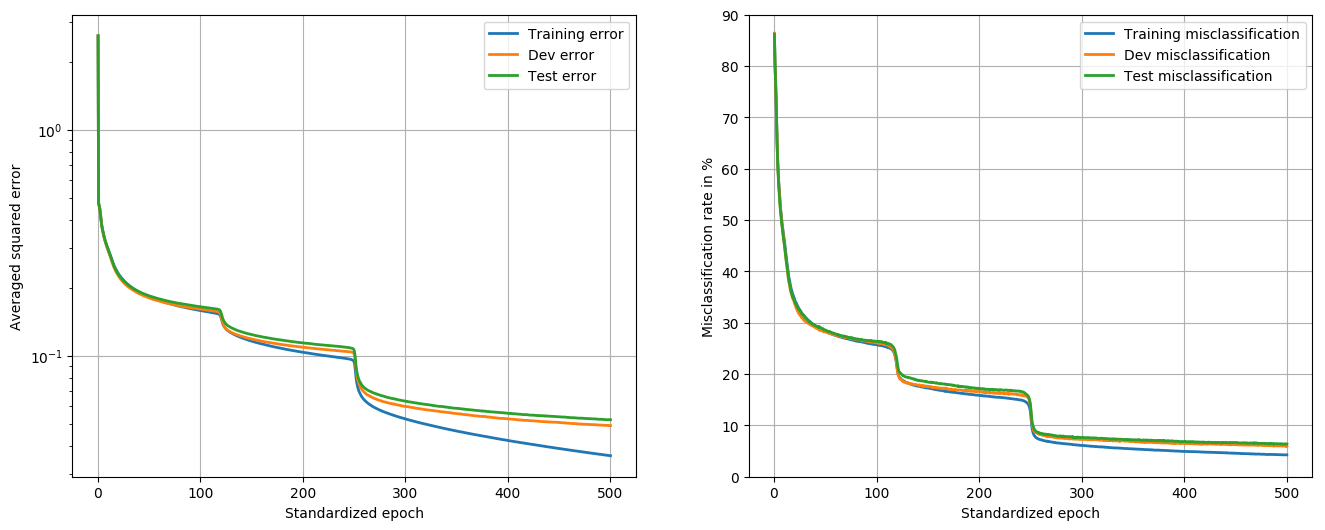
\includegraphics[width=\linewidth]{./Problem_3/Problem_3.1_0.1_500_sigm.png}
			\caption{Squared loss and misclassification error for the one layer hidden network with sigmoid transfer functions. I chose displaying the misclassification over a wider range since there are some interesting features happening above $20\%$.}
			\label{fig:sigmoid}
		\end{figure}
		\item In figure \ref{fig:sigmoid_weights} ten weights for the hidden layer are visualized. One can not really guess what is displayed and I expected that those pixel in the corners and on the edges mostly should be dark (small weights) since they do not carry much information for predicting the digit and the pixel in the center might would be brighter in general. This is not the case here. 
		\begin{figure}[h]
			\centering
			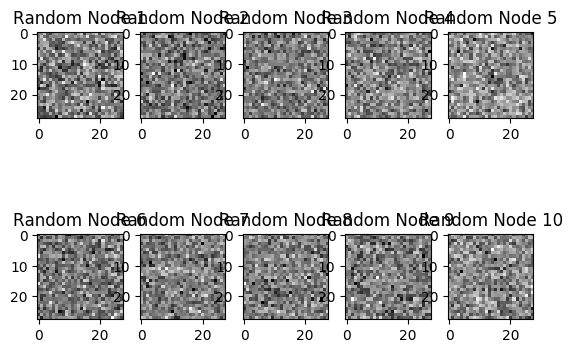
\includegraphics[width=\linewidth]{./Problem_3/Problem_3.1_0.1_500_weights_sigm.png}
			\caption{Visualization of the weights for ten nodes in the hidden layer after sigmoid transfer.}
			\label{fig:sigmoid_weights}
		\end{figure}
	\end{enumerate}
	\item 
	\begin{enumerate}[label=(\alph*)]
		\item 
		Since I had a really hard time to get the relu function working I decided, according to the instructor's post on the class canvas, to use relu only for the input layer and to use sigmoid for the second layer. For running gradient descent I used pytorch and built a one layer hidden network with 100 hidden nodes, a minibatch size of $200$, trained for $500$ epochs, used a constant step size of $0.1$ and no regularization. The weights are initialized by picking values from a normal distribution between zero and one. 	
		\item 
		For larger stepsizes than $0.1$ or $1$ we do not really find a decrease in error rate. The error does not diverge since we limit our output and the transfers with the sigmoid and relu functions which are limited between $0$ ($-1$) and $1$. 	
		\item See figure \ref{fig:relu}
		\item See figure \ref{fig:relu}. The lowest test error achieved is around $16\%$. Due to some unknown reasons I could achieve a better error and I hadn't had time or computational power to test a wider range of parameters.
		\begin{figure}[h]
			\centering
			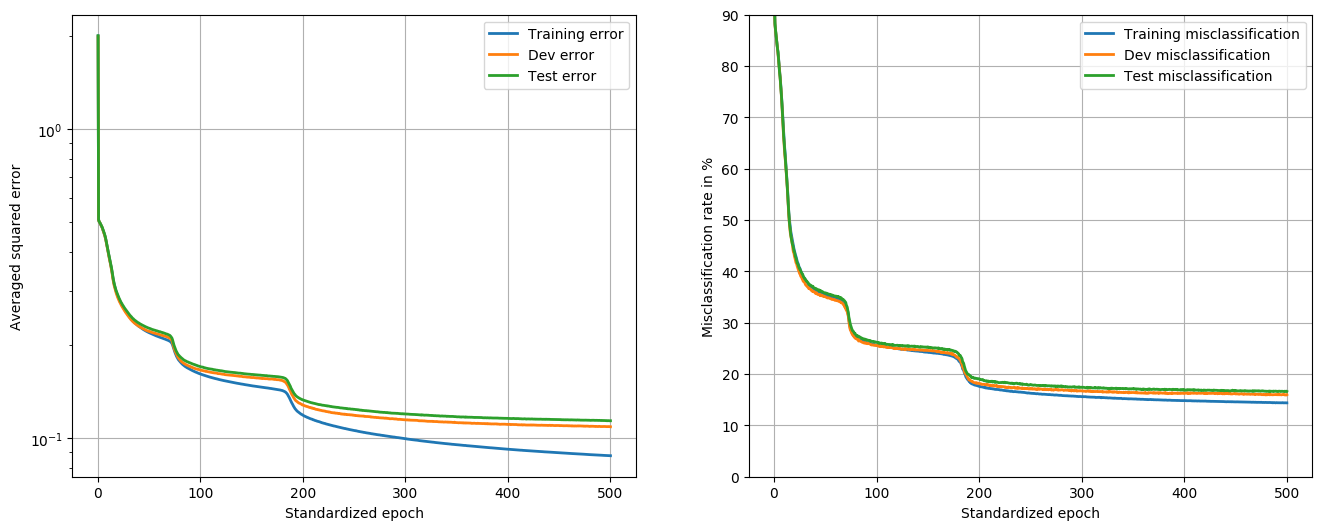
\includegraphics[width=\linewidth]{./Problem_3/Problem_3.1_0.1_500_relu.png}
			\caption{Squared loss and misclassification error for the one layer hidden network with sigmoid transfer functions. I chose displaying the misclassification over a wider range since there are some interesting features happening above $20\%$.}
			\label{fig:relu}
		\end{figure}
		\item In figure \ref{fig:relu_weights} ten weights for the hidden layer are visualized. One can not really guess what is displayed and I expected that those pixel in the corners and on the edges mostly should be dark (small weights) since they do not carry much information for predicting the digit and the pixel in the center might would be brighter in general. This is not the case here. 
		\begin{figure}[h]
			\centering
			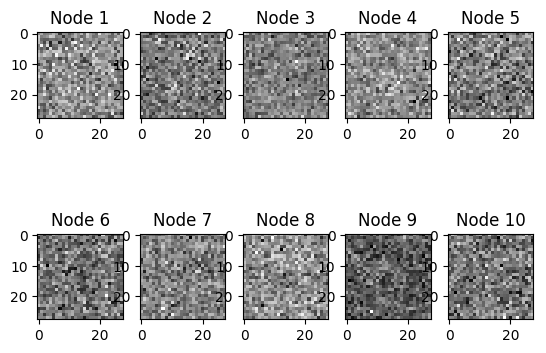
\includegraphics[width=\linewidth]{./Problem_3/Problem_3.1_0.1_500_weights_relu.png}
			\caption{Visualization of the weights for ten nodes in the hidden layer after relu transfer.}
			\label{fig:relu_weights}
		\end{figure}
	\end{enumerate}
	
\end{enumerate}

%\chapter*{Bibliography}
\addcontentsline{toc}{chapter}{Bibliography}%	


\bibliographystyle{unsrt}
\bibliography{./bib}
/


\end{document}  